
\section{Ergänzungen}

\begin{frame}
    \frametitle{\acp{TEA} und \acp{CbCC} Ursache}

    \begin{itemize}
        \item moderne \acp{CPU} sind hochkomplexe Maschinen
        \item mathematische Modelle der theoretischen Informatik werden simuliert
        \item tatsächliche Berechnungen werden durch abweichende Modelle optimiert
        \item Beispiele sind spekulative- und \ac{OoO}-Execution, sowie Cache selbst
        \item Nutzen dieser Konzepte zum Ableiten unzugänglicher Informationen
    \end{itemize}

    \pause

    \begin{block}{Die Folgen}
        \acp{TEA} und \acp{CbCC} stellen genauso wie Side-Channel
        eine fundamentale Schwachstelle in modernen Computersystemen
        dar. Sie können vollständig ohne physischen Zugriff ausnutzt
        werden, obwohl Konzepte der Hardware die Ursache für die
        Schwachstellen sind.
    \end{block}

\end{frame}

\begin{frame}
    \frametitle{Verschiedene Angriffe}

    \begin{minipage}[c][0.5\textheight][b]{\textwidth}
        \begin{center}
            \scriptsize
            \begin{tikzpicture}
                \node at (0,5) {
                    \begin{chronology}[5]{2015}{2030}{0.9\textwidth}
                        \event[\decimaldate{1}{11}{2017}]{2020}{\alt<1,4>{\textbf{Spectre \cite{kocher_spectre_2019} \& Meltdown \cite{lipp_meltdown_2020}}}{Spectre \cite{kocher_spectre_2019} \& Meltdown \cite{lipp_meltdown_2020}}}
                        \event[\decimaldate{1}{11}{2024}]{\decimaldate{1}{4}{2025}}{\alt<2,4>{\textbf{SLAP \cite{kim_slap_2025} \& FLOP \cite{kim_flop_2025}}}{SLAP \cite{kim_slap_2025} \& FLOP \cite{kim_flop_2025}}}
                        \event[\decimaldate{1}{9}{2025}]{\decimaldate{1}{2}{2026}}{\alt<3,4>{\textbf{RAIN (L1TF Reloaded) \cite{hertogh_rain_nodate}}}{RAIN (L1TF Reloaded) \cite{hertogh_rain_nodate}}}
                        %\event{\decimaldate{25}{12}{2001}}{three}
                    \end{chronology}
                };
            \end{tikzpicture}
        \end{center}
    \end{minipage}

    \vspace{0.25cm}

    \begin{minipage}[t][0.5\textheight][t]{\textwidth}
        \only<1>{
            \begin{itemize}
                \item Spectre und Meltdown wurden von verschiedenen Teams entdeckt
                \item nutzen beide Transient Execution und \ac{CbCC} aus
                \item maßgeblich für grundsätzlich zwei Arten von Angriffen (spekulative- vs \ac{OoO}-Execution)
                \item Meltdown nutzt ein vom Angreifer kontrolliertes Gadget, Spectre teilweise
            \end{itemize}
            \note{- Spectre \& Meltdown Ende 2017 bis 2020 entdeckt und veröffentlicht}
            \note{- stellen neue Art von Angriff mit Transient Execution dar}
            \note{- Kategorisierung aller Angriffe in spekulative Ausführung oder OoO-Execution}
            \note{- Meltdown wird Code vollständig vom Angreifer kontrolliert, Spectre je nach Variante unterschiedlich}
        }
        \pause
        \only<2>{
            \begin{itemize}
                \item ausnutzen neuer Predictoren (Load Adress/Value Prediction)
                \item ähnlich wie iLeakage \cite{kim_ileakage_2023} umgehen der
                Apple-Webkit Sandbox für willkürliches lesen von Speicher
                \item lange Laufzeit durch Verstärken von Laufzeitunterschieden
                \item nur so lange möglich wie Browser Fenster offen\\
                \textrightarrow\space Dauer des Angriffs hat Einfluss auf Erfolg
            \end{itemize}
            \note{- LAP \& LVP -> erster Nachweis + Exploit}
            \note{- zukünftig weitere Verbreitung solcher Predictoren?}
            \note{- "Vorgänger" iLeakage (Spectre-Angriff mit anderem Predictor + Timing Amplification)}
            \note{- Lesen von Speicher innerhalb des Browser-Prozess -> SLAP und FLOP deutlich begrenzt, aber möglich}
            \note{- Laufzeit recht hoch, Nutzer darf Tab nicht schließen + Angreifer öffnet Ziel Webseite}
        }
        \pause
        \only<3>{
            \begin{itemize}
                \item Verwendung von L1TF \cite{bulck_foreshadow_2018} in Kombination mit einem half-spectre Gadget
                \item Auslesen von Speicher des Hypervisor Hosts innerhalb einer \ac{VM}
                \item umgeht bisherige Mitigationen \textrightarrow\space zugrunde liegendes Problem bleibt bestehen
                \item Laufzeit in Public Clouds eher irrelevant
            \end{itemize}
            \note{- L1TF Angriff von 2018 -> wurde „quasi“ Mitigiert}
            \note{- L1TF Reloaded nutzt half-spectre Gadget + L1TF}
            \note{- half-spectre = spekulatives Laden eines Secrets (out of bound), ohne Adressen abhängig von Wert zu laden}
            \note{- Gadget lädt beliebige Adresse (out of bound) in Cache -> lesen während Transient Execution mit L1TF}
            \note{- Konkreter Exploit: Auslesen von Hypervisor Memory in KVM (Public Cloud) -> Laufzeit weniger relevant, da unbegrenzt Zeit}
        }
        \pause
        \only<4>{
            \begin{itemize}
                \item Gadget für Encodierung in den \ac{CbCC} häufig von Angreifer kontrolliert\\
                \textrightarrow\space Encodierung und Technik kann frei gewählt werden
                \item Relevanz der Laufzeit für allgemeines Risiko solcher Angriffe
                \item teilweise relevant für Frage der Umsetzbarkeit
            \end{itemize}
            \note{- viele Angriffe mit Angreifer kontrolliertem Gadget (alle hier gezeigten)}
            \note{- CbCC kann frei gewählt werden -> neben Technik besonders Encodierung}
            \note{- Laufzeit für Risiko eines konkreten Angriffs relevant}
            \note{- Frage praktische Umsetzbarkeit bei sehr hoher Laufzeit}
        }
    \end{minipage}

\end{frame}

\begin{frame}
    \frametitle{Messungen}

    \only<1>{
        \begin{itemize}
            \item Ziel ist grundsätzlicher Vergleich von bitweiser und Array-Index Encodierung
            \item Ausführung einzelner Übertragungen semi-zufälliger Eingabewerte
            \item unterschiedlicher Stride, Anzahl Bit, Trainingsläufe
            \item Speichern der Laufzeit, Eingabe, Ausgabe, Stride, Anzahl Bit, Trainingsläufe
        \end{itemize}

        \note{- Ziel an sich bitweise Encodierung zu demonstrieren und mit Array-Index zu vergleichen}
        \note{- entwickeltes Programm führt eine Übertragung von Eingabewert mit angegebener Encodierung durch}
        \note{- Eingabe semi zufälliger Werte zum übertragen (Randomisierung anhand von Index -> jedes Mal gleiche Werte)}
        \note{- Ausführung über 100 Iterationen je Parameter-Kombination}
        \note{- Parameter: Stride, Anzahl übertragener Bit, Anzahl Trainingsläufe}
    }

    \pause

    \begin{columns}
        \begin{column}{0.49\textwidth}
            \only<2>{
                \textbf{Auffälligkeiten bitweise}
                \begin{itemize}
                    \item steigende Genauigkeit bei unter $20$ Trainingsläufen (im Gegensatz zu Array-Index)
                    \item schon bei niedrigem Stride hohe Genauigkeit (ab etwa $2^8$)
                    \item Genauigkeit gegenüber Array-Index ähnlich, aber grundsätzlich schlechter
                \end{itemize}
            }
            \only<3>{
                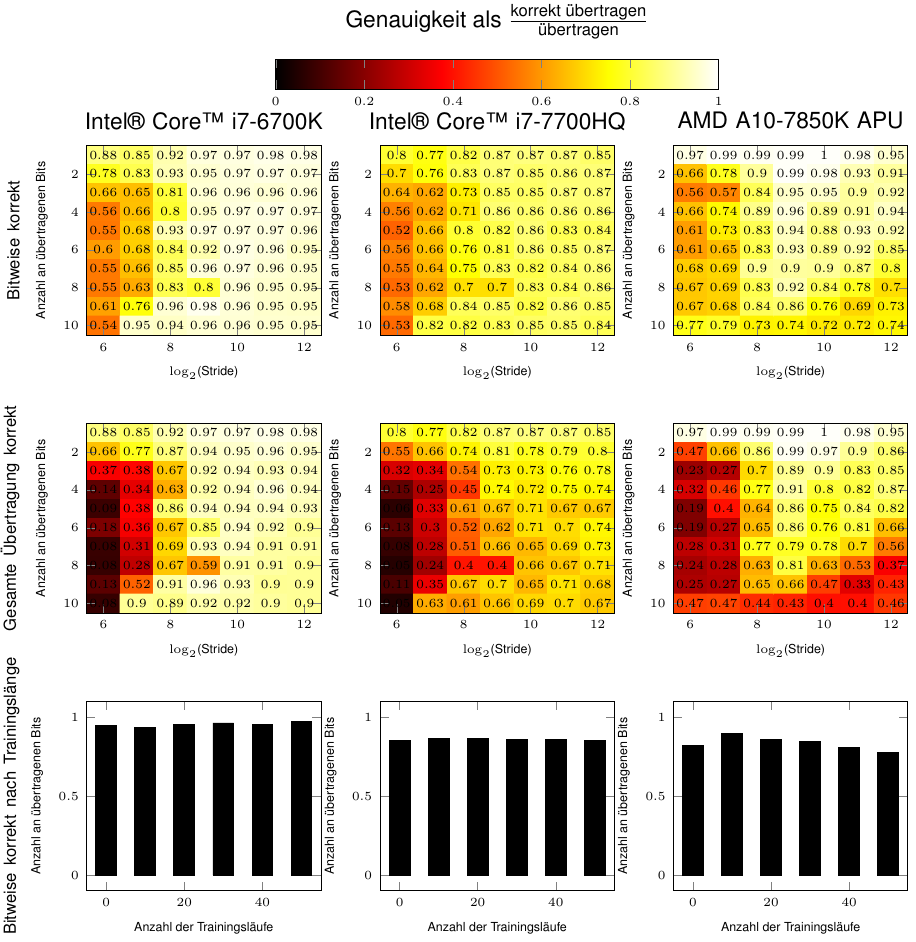
\includegraphics[width=\textwidth]{img/statistic_array-index.png}
            }
        \end{column}
        \begin{column}{0.49\textwidth}
            \only<2>{
                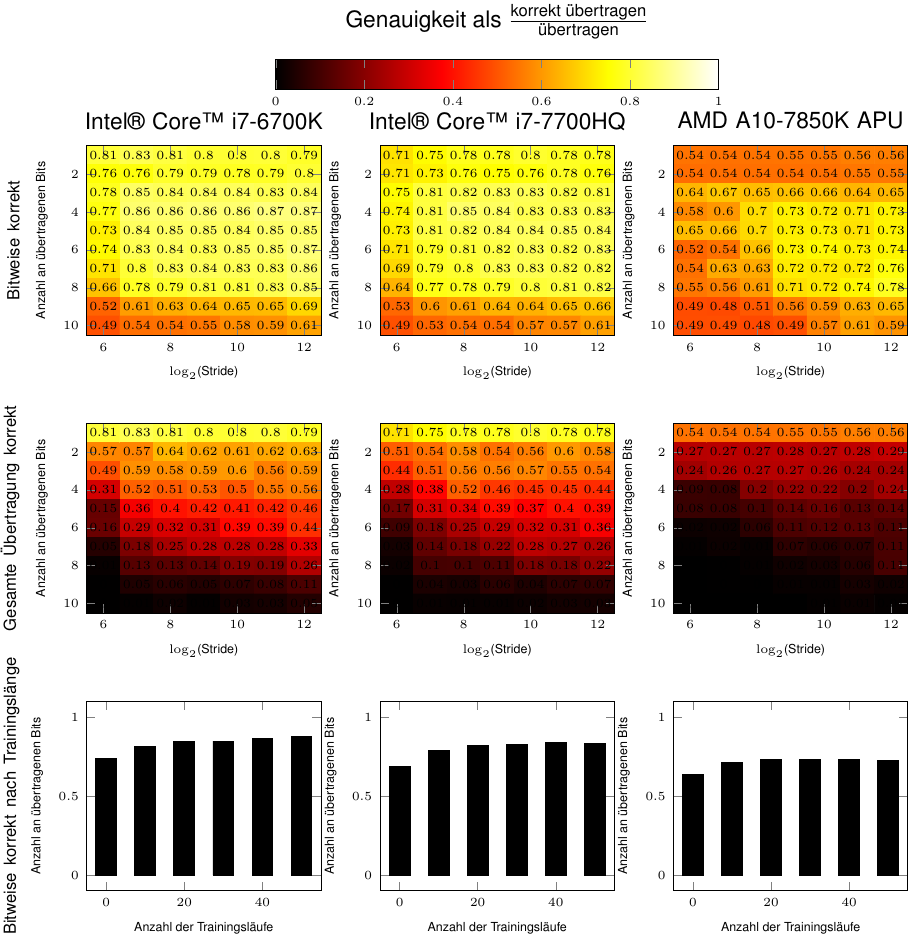
\includegraphics[width=\textwidth]{img/statistic_bitwise.png}
            }
            \only<3>{
                \textbf{Auffälligkeiten Array-Index}
                \begin{itemize}
                    \item sehr hohe Genauigkeit, auch mehr als 10 Bit
                    \item Trainingsläufe kein Einfluss auf Genauigkeit
                    \item inkonsistente Ergebnisse je nach Hardware
                \end{itemize}
            }
        \end{column}
    \end{columns}

    \only<2>{
        \note{- BITWEISE:}
        \note{- wie erwartet gute Genauigkeit bis Bitanzahl (Limit durch Anzahl Instruktionen)}
        \note{- Bis etwa 20 Trainingsläufe steigt Genauigkeit -> logisch wegen Predictor -> bei Array-Index nicht der Fall??}
        \note{- auch bei niedrigem Stride gute Genauigkeit, ab recht niedrigem Stride konstant}
        \note{- Übertragung wie bei Array-Index klar erkennbar, grundsätzlich schlechtere Genauigkeit}
    }
    \only<3>{
        \note{- ARRAY-INDEX:}
        \note{- Sehr sehr hohe Genauigkeit mit deutlich über 90\% korrekten Übertragungen}
        \note{- wie erwartet keine Limitierung Bit Anzahl, Vergleich bitweise}
        \note{- hier keine konsistenter Einfluss von Trainingsläufen auf Genauigkeit erkennbar}
        \note{- Ergebnisse des AMD A10 Prozessors sehr auffällig -> 100\% bei 1 bit, geringere Genauigkeit mit steigendem Stride, höchste Genauigkeit bei geringerem Stride?? etc.}
    }
    \pause

\end{frame}